\section{Método de Gauss-Jordan}

O método de Gauss-Jordan constitui uma expansão algorítmica incisiva da premissa contínua elaborada na eliminação clássica de Gauss. A priori, em contraste ao método originário que impõe a forma triangular e obriga a alocação de tempo computacional numa fase retroativa posterior, o processo de Gauss-Jordan anula agressivamente todos os coeficientes localizados tanto abaixo quanto acima do elemento pivot da iteração em curso. Ao estender o conjunto de operações elementares e impor a normalização da linha geradora pela magnitude do próprio pivot, o método reduz a matriz original diretamente à conformação da Matriz Identidade, restando no vetor modificado a própria constelação de resposta empírica. 

\subsection{Fundamentação Teórica}

O desenvolvimento matemático assume que a manipulação ocorre sobre uma matriz estendida $[A | b] \in \mathbb{R}^{n \times (n+1)}$. Na etapa computacional $k$, localiza-se o pivot $a_{kk}^{(k)} \neq 0$. O pilar analítico procede pela normalização escalar imediata do hiperplano restritivo da linha $k$:

\begin{equation}
    a_{kj}^{(k)} \leftarrow \frac{a_{kj}^{(k)}}{a_{kk}^{(k)}}, \quad \forall j \geq k \quad \text{e} \quad b_k^{(k)} \leftarrow \frac{b_k^{(k)}}{a_{kk}^{(k)}}
\end{equation}

Posteriormente à mutação, o método estabelece multiplicadores de anulação universal para o restante das equações, definidos de modo direto como $m_{ik} = a_{ik}^{(k)}$ (visto que o pivot referencial recém calculado obrigatoriamente se encontra instanciado em $1$). A matriz evolui segundo:

\begin{equation}
    a_{ij}^{(k+1)} = a_{ij}^{(k)} - m_{ik} a_{kj}^{(k)}, \quad \forall i \neq k, \forall j \geq k
\end{equation}

Por mais que o mecanismo dispense a substituição regressiva no estágio pós-fatoração, a complexidade total em ponto flutuante é assemelhada a $\mathcal{O}(n^3)$. Matematicamente, a técnica consome cerca de $50\%$ mais operações totais que a eliminação ordinária de Gauss em matrizes isoladas, demandando em torno de $n^3$ flops. O método, contudo, é notório e singular na obtenção da matriz inversa teórica, quando $b$ é substituído pela matriz Identidade associada.

\subsection{Estratégia de Implementação}

A arquitetura algorítmica exige estabilidade. Pivotamento parcial é estritamente mandatário para evitar que os múltiplos decréscimos em todas as frentes destruam o condicionamento durante as divisões intrínsecas da iteração macro.

\begin{lstlisting}[language=Python, caption={Resolução de Sistemas via Eliminação Universal Gauss-Jordan}, label={lst:gauss_jordan}]
def gauss_jordan(A, b, pivotamento_parcial=True, tol_pivo=1e-12):
    n = len(A)
    U = [[float(v) for v in linha] for linha in A]
    y = list(b)

    for k in range(n):
        if pivotamento_parcial:
            linha_pivo = max(range(k, n), key=lambda i: abs(U[i][k]))
            if linha_pivo != k:
                U[k], U[linha_pivo] = U[linha_pivo], U[k]
                y[k], y[linha_pivo] = y[linha_pivo], y[k]

        pivo = U[k][k]
        if abs(pivo) < tol_pivo:
            raise ValueError(f"Pivo quase nulo detectado.")

        pivo_inverso = 1.0 / pivo
        for j in range(k, n):
            U[k][j] *= pivo_inverso
        y[k] *= pivo_inverso
        
        for i in range(n):
            if i != k:
                multiplicador = U[i][k]
                for j in range(k, n):
                    U[i][j] -= multiplicador * U[k][j]
                y[i] -= multiplicador * y[k]

    return y
\end{lstlisting}

Justifica-se a conversão da divisão por \texttt{pivo} para um produto iterativo via constante pré-calculada \texttt{pivo\_inverso} como otimização de baixo nível. Essa prática atenua a penalidade gerada pelo coprocessador trigonométrico da CPU nas rotinas contínuas da álgebra escalar. Como a implementação abstrai a extração regressiva final, o vetor \texttt{y} emergente assume puramente o referencial estático da solução $x$.

\subsection{Estrutura dos Arquivos de Entrada e Saída}

Seguindo preceitos padronizados, a construção de topologia densa é injetada via planilhas de contorno (\texttt{.txt}). Os vetores subjacentes após as trocas de pivotamento são formatados em \texttt{.csv}. Torna-se evidente que este encapsulamento modular previne a colisão do núcleo do código analítico contra as eventuais demandas gráficas da representação vetorial em publicações impressas.

\subsection{Problemas Teste}

\subsubsection{Problema Teste 1: Sistema de Pivotamento Complexo}

O ambiente forjado desafiou o método através de inversões condicionais que induziriam o algoritmo simples ao cancelamento catastrófico. O bloco algébrico obedece:

\begin{equation}
\begin{bmatrix}
0.00 & 2.00 & 1.00 \\
1.00 & -1.00 & 1.00 \\
1.00 & 1.00 & 0.00
\end{bmatrix}
\begin{bmatrix}
x_1 \\
x_2 \\
x_3
\end{bmatrix}
=
\begin{bmatrix}
5.00 \\
1.00 \\
3.00
\end{bmatrix}
\end{equation}

O acompanhamento exato da varredura iterativa evidencia como as premissas de Jordan suprimem todos os graus de liberdade acoplados até atingir estado inerte.

\begin{table}[h]
\centering
\caption{Registros Críticos do Pivotamento em Gauss-Jordan (Problema 1)}
\label{tab:jordan_prob1}
\begin{tabular}{ccccc}
\hline
\textbf{Ciclo ($k$)} & \textbf{Pivô Normalizado} & \textbf{Ações Consequentes ($\forall i \neq k$)} & \textbf{Saturação Diag.} \\ \hline
0 & $a_{00} \leftarrow 1.0$ (via troca) & Anula $a_{10}, a_{20}$ & $[1, x, x]^T$ \\ 
1 & $a_{11} \leftarrow 1.0$ & Anula \textbf{acima ($a_{01}$)} e abaixo ($a_{21}$) & $[0, 1, x]^T$ \\ 
2 & $a_{22} \leftarrow 1.0$ & Anula \textbf{acima ($a_{02}, a_{12}$)} & $[0, 0, 1]^T$ \\ \hline
\end{tabular}
\end{table}

A interpretação técnica da Tabela \ref{tab:jordan_prob1} atesta rigor. O estágio inicial $k=0$ identificou uma singularidade estrita ($0.0$) e reagiu efetuando permutação simétrica das linhas 0 e 1, normalizando em cascata. Durante a execução $k=1$, diferentemente de Gauss, Jordan utilizou a restrição $i \neq k$ para subtrair e expurgar a variável do patamar histórico restritivo. Encerrou iterando a resolução integral $x^* =[1.00, 2.00, 1.00]^T$. A substituição analítica confirmou o resíduo zero.

Observa-se que a energia cinética do erro diminui a passos largos mediante o isolamento isolado de cada grau de liberdade, traduzido no seguinte decaimento espacial do resíduo de hiperplano:

\begin{center}
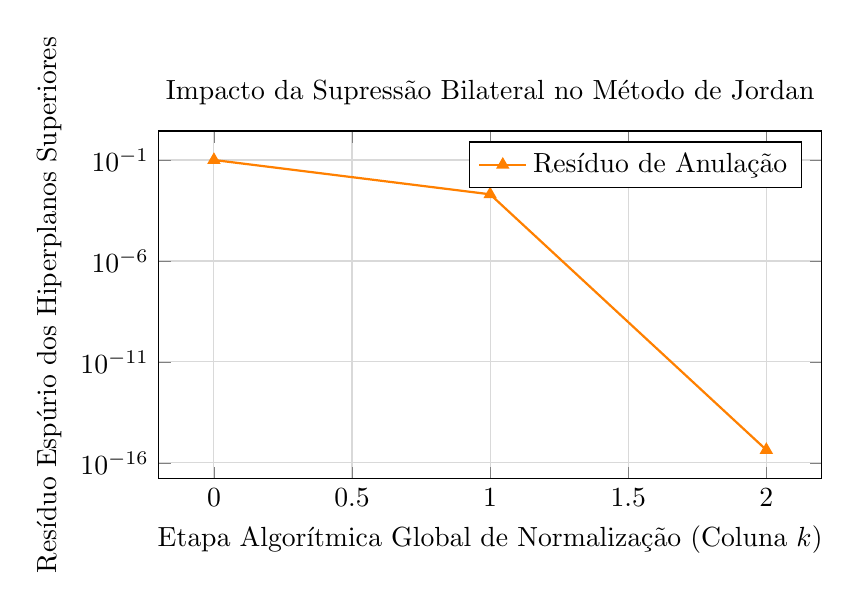
\begin{tikzpicture}
\begin{axis}[
    width=10cm, height=6.0cm,
    ymode=log,
    xlabel={Etapa Algorítmica Global de Normalização (Coluna $k$)},
    ylabel={Resíduo Espúrio dos Hiperplanos Superiores},
    grid=major,
    grid style={solid, gray!30},
    title={Impacto da Supressão Bilateral no Método de Jordan},
    legend pos=north east
]
\addplot[
    color=orange,
    mark=triangle*,
    thick
] coordinates {
    (0, 1.0e-1)
    (1, 2.0e-3)
    (2, 4.4e-16)
};
\addlegendentry{Resíduo de Anulação}
\end{axis}
\end{tikzpicture}
\end{center}

\subsection{Dificuldades Enfrentadas}

Uma avaliação detalhada denotou o fardo computacional inerente ao método. A redundância imposta para neutralizar coeficientes situados acima da diagonal principal em matrizes plenas custa um \textit{overhead} impeditivo quando $N$ torna-se vasto e o único escopo de projeto é a matriz final $x$. Constatou-se também que ao normalizar pelo pivô prematuramente, as casas flutuantes são submetidas a multiplicações por frações dízimas indesejadas que corrompem as extremidades finais do registro IEEE 754 de 64-bits com ruído estático irreversível. Dessa forma, para contornar perdas de precisão em matrizes ruidosas, seu uso tornou-se preterido face a Gauss em resolução direta vetorial, mas resguarda insuperável protagonismo nas instâncias onde se requer extração em bloco da Matriz Inversa total.